\documentclass[11pt,letterpaper]{article}
\usepackage[T1]{fontenc}
\usepackage[utf8]{inputenc}
\usepackage{lmodern}
\usepackage[margin=1in]{geometry}
\usepackage{graphicx}
\usepackage{booktabs}
\usepackage{tabularx}
\usepackage{float}
\usepackage{amsmath}
\usepackage[table]{xcolor}
\usepackage{enumitem}
\usepackage{caption}
\usepackage{tikz}
\usetikzlibrary{positioning,arrows.meta,shapes.geometric}
\usepackage[hidelinks]{hyperref}
\setlist{nosep,leftmargin=1.3em}
\captionsetup{font=small,labelfont=bf}
\graphicspath{{figures/}}
\newcommand{\best}[1]{\textbf{#1}}

\title{Forecasting August 2026 Food-Shelf Activity in Minnesota\\[2pt]
\large MinneMUDAC 2026 --- Question 7: Methods, Validation, and Submission}
\author{MinneMUDAC 2026 Undergraduate Team}
\date{Information cutoff: July 31, 2026}

\begin{document}
\maketitle
\sloppy

\begin{abstract}
\noindent
We forecast August 2026 visits (HouseholdsReg), pounds distributed (PoundsReg), and
individuals served (IndividualsReg) for each of Minnesota's 87 counties using only information
available on or before July 31, 2026. We first backtested the five reference models specified in the
question, then ran a multi-agent study in which four specialist workflows (statistical, panel
machine learning, deep learning and foundation models, and structural/data-quality) built 101 model
variants that were all scored by one shared, leakage-safe harness. Many sophisticated models beat
the seasonal-naive baseline on the historical record, but none did so with statistical significance,
and an out-of-sample replay of ``pick the best model'' performed worse than simple methods. We
therefore built the forecast from a small set of robust county-level methods (seasonal naive,
damped year-over-year growth, per-county local-model selection, their blend, and a recent
three-month mean), letting \emph{each county} use the method that tracked it best over the
previous twelve months. Against the plain blend, this county-by-county selection lowers county-level
WAPE from 10.7\% to 9.5\% (visits), 10.8\% to 8.9\% (pounds), and 10.6\% to 9.1\% (individuals)
across 31 rolling one-month-ahead tests, removes systematic under-forecasting, and is
significantly better in paired tests. The submission implies statewide totals of 237{,}861 visits,
12.99 million pounds, and 738{,}532 individuals, and it cuts county-level error relative to seasonal
naive by about 40\%.
\end{abstract}

\section{Task and information cutoff}
Question 7 asks for an August 2026 forecast under a strict information cutoff of July 31, 2026, for
every internal and external feature, with the prediction pipeline kept in a separate folder and an
explicit cutoff check. The submission format requires one row per county with three predicted
quantities. Table~\ref{tab:defs} maps them to the prepared data.

\begin{table}[H]\centering\small
\caption{Submission targets and their source fields.}\label{tab:defs}
\begin{tabular}{lll}
\toprule
Submission column & Prepared field & Source field \\
\midrule
\texttt{HouseholdReg\_Predicted} & \texttt{visits} & \texttt{HouseholdsReg} \\
\texttt{PoundsReg\_Predicted} & \texttt{pounds} & \texttt{PoundsReg} \\
\texttt{IndividualsReg\_Predicted} & \texttt{individuals} & \texttt{IndividualsReg} \\
\bottomrule
\end{tabular}
\end{table}

\paragraph{Cutoff enforcement.} The cutoff is enforced in code rather than by convention:
\begin{enumerate}
  \item The loader refuses to run if the source file contains any month after July 2026.
  \item Every forecast receives a data slice that ends exactly one month before its target; this is
        asserted on each of the $\sim$10{,}000 model calls in the study.
  \item Backtest actuals are looked up only after a prediction has been produced.
  \item Any tuning (window length, damping, local-model choice) is done inside the slice, using only
        earlier months; no parameter was tuned against backtest scores.
  \item No external predictors are used in the submitted model. SNAP, poverty, and Map the Meal Gap
        variables were excluded because their release dates could not be verified or they are
        annual and cannot inform a single month.
\end{enumerate}

\paragraph{Data policy.} We use the project's prepared site-month file
(\texttt{Data/processed/}\allowbreak\texttt{foodshelf\_site\_month.csv}), which resolves documented duplicates and
clear typographical errors. All observations flagged as high outliers or as households exceeding
individuals are retained; the policy was locked before model selection and a sensitivity check
(Section~\ref{sec:diag}) shows these rows change August growth by less than 0.4 percentage points
in 2024--25. Wilkin County has no food-shelf site in the data and is predicted as zero.

\section{Data and diagnostics}\label{sec:diag}
Statewide monthly totals span January 2022--July 2026 (55 months). Figure~\ref{fig:series} shows two
regimes: a strong ramp-up through mid-2023 (visits rose from about 124k to 237k per month) and a
roughly flat level since 2024.

\begin{figure}[H]\centering
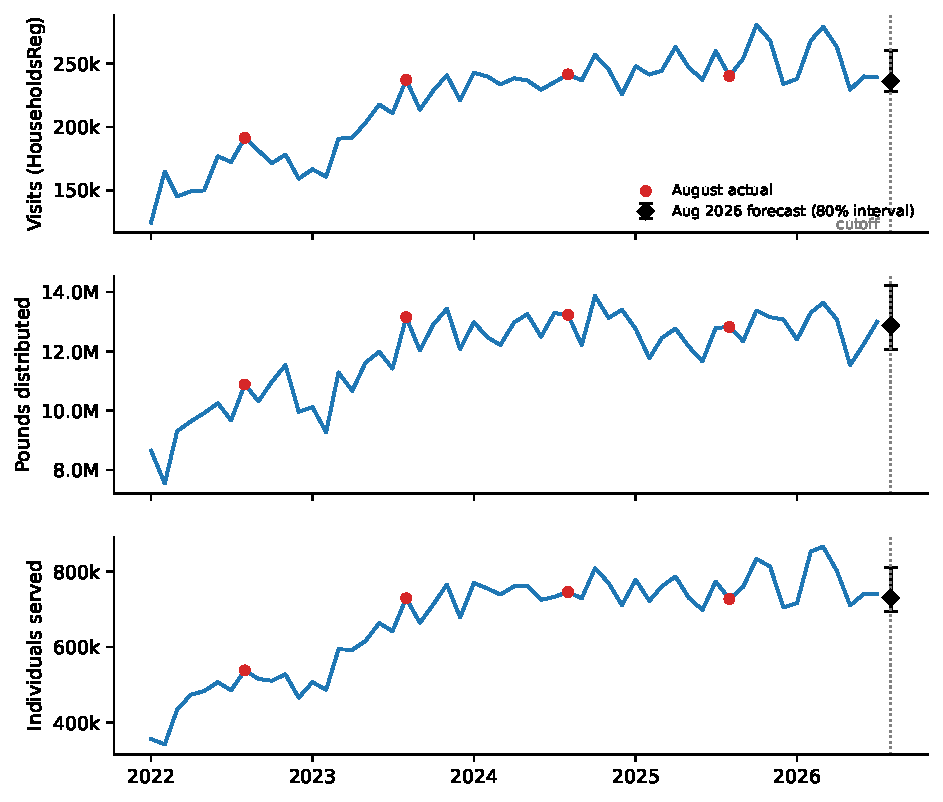
\includegraphics[width=0.85\textwidth]{statewide_series.pdf}
\caption{Statewide monthly outcomes with August values (red), the July 31, 2026 cutoff (dotted), and
the August 2026 forecast with an empirical 80\% interval.}\label{fig:series}
\end{figure}

\paragraph{Is July 2026 complete?} Because every model leans on the most recent months, we checked
for late or partial reporting. July 2026 had 462 reporting sites (0.99 of the prior three-month
mean, inside the normal 0.97--1.04 band), 98.3\% of June reporters also reported in July (equal to
the 2024--26 average), and the share of sites with sudden drops was at the low end of history.
The 8\% year-over-year fall in July visits is real: it comes from sites present in both years, and
July 2025 was itself an unusual spike driven by about ten sites.

\paragraph{Where growth came from.} A shift-share decomposition shows that the 2023 and 2024
growth (+26.4\% and +15.3\% in visits) was almost entirely same-site growth, not new sites
(Figure~\ref{fig:sites}, left). In 2026 year-to-date, visits are up 0.9\%, pounds 3.4\%, and
individuals 4.1\%, and the most recent three months show visits down 4.8\%.

\paragraph{August seasonality is unstable.} The August/July ratio fell from 1.11--1.13 in 2022--23 to
1.03 in 2024 and 0.92 in 2025 (Figure~\ref{fig:sites}, right). The large early ratios were produced by
the growth regime, which is why ``July times a historical ratio'' forecasts perform poorly.

\begin{figure}[H]\centering
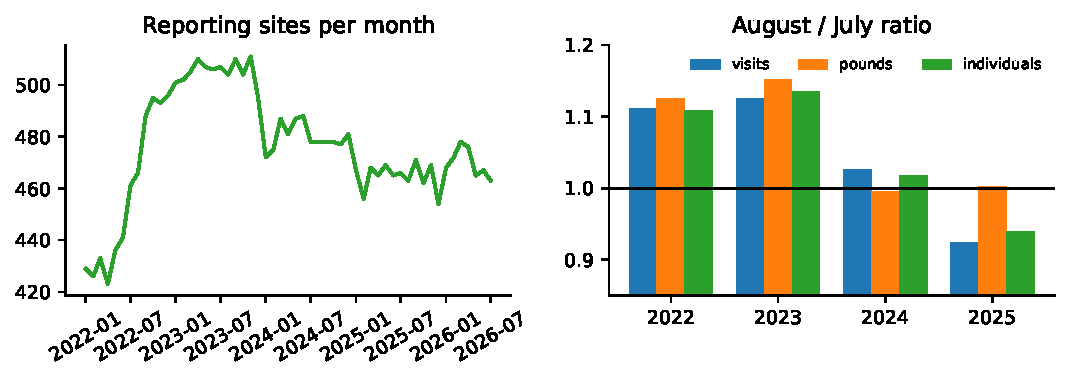
\includegraphics[width=0.9\textwidth]{sites_and_ratio.pdf}
\caption{Left: reporting sites per month. Right: August/July ratio by year and outcome.}\label{fig:sites}
\end{figure}

\section{Validation design}
Only three historical Augusts can be used as holdouts, too few to choose among many models. We
therefore used two protocols with the same one-month horizon as the real task:
\begin{description}
  \item[Protocol A (official).] Forecast August 2023, 2024, and 2025 using data through July 31 of
        each year.
  \item[Protocol B (robustness).] Forecast each month from January 2024 to July 2026 one step ahead
        (31 origins).
\end{description}
The August 2023 fold sits inside the ramp-up regime and has only 19 months of history; it is
reported, but we also show the 2024--25 average. Our main error measure is the mean absolute
percentage error (MAPE); at county level we use the weighted absolute percentage error
$\text{WAPE}=\sum_c|\hat y_c-y_c|/\sum_c y_c$, because small counties make ordinary MAPE unstable.

Before any agent results were seen, we wrote down a selection rule. A challenger would replace
seasonal naive only if it (i) lowered Protocol B MAPE by at least one point, (ii) lowered Protocol A
MAPE, (iii) was no more than 1.5 points worse on the 2024--25 Augusts, and (iv) never failed to
produce a forecast.

\section{The five reference models}
Table~\ref{tab:required} and Figure~\ref{fig:required} report the five models specified in the
question, plus the damped year-over-year model (last August $\times$ $(1+0.5(g-1))$, where $g$ is
the growth of the latest three months over the same months a year earlier).

\begin{table}[H]\centering\small
\caption{Reference models: August MAPE (\%) over 2023--25, per-fold APE, and Protocol B MAPE.}\label{tab:required}
\begin{tabular}{llrrrrr}
\toprule
Outcome & Model & Aug MAPE & 2023 & 2024 & 2025 & Monthly \\
\midrule
Visits & Seasonal naive & 7.20 & 19.36 & 1.75 & \best{0.49} & 8.52\\
 & YTD growth & 9.02 & \best{0.07} & 21.33 & 5.66 & 9.06\\
 & July $\times$ Aug/Jul ratio & 10.14 & 1.29 & 8.95 & 20.19 & 7.36\\
 & Trend + month regression & 13.06 & 3.77 & 15.24 & 20.17 & 8.72\\
 & Robust median ensemble & 9.18 & 2.53 & 12.10 & 12.91 & 6.01\\
 & Damped YoY & \best{5.28} & 8.62 & 3.66 & 3.57 & \best{5.43}\\
\midrule
Pounds & Seasonal naive & 7.03 & 17.25 & \best{0.61} & 3.23 & 6.59\\
 & YTD growth & 6.68 & 2.74 & 16.71 & 0.60 & 6.14\\
 & July $\times$ Aug/Jul ratio & 9.65 & \best{2.32} & 14.34 & 12.29 & 8.71\\
 & Trend + month regression & 10.21 & 4.87 & 11.19 & 14.55 & 8.90\\
 & Robust median ensemble & 8.11 & 3.80 & 12.77 & 7.76 & 6.05\\
 & Damped YoY & \best{5.06} & 10.06 & 5.08 & \best{0.02} & \best{5.16}\\
\midrule
Individuals & Seasonal naive & 10.32 & 26.15 & \best{2.25} & 2.56 & 8.75\\
 & YTD growth & 9.79 & \best{1.79} & 24.91 & 2.68 & 9.79\\
 & July $\times$ Aug/Jul ratio & 10.17 & 2.40 & 10.23 & 17.89 & 8.07\\
 & Trend + month regression & 15.49 & 6.20 & 17.31 & 22.97 & 12.27\\
 & Robust median ensemble & 9.45 & 4.30 & 13.77 & 10.28 & 6.71\\
 & Damped YoY & \best{7.50} & 15.02 & 5.34 & \best{2.15} & \best{5.86}\\
\bottomrule
\end{tabular}
\end{table}

\begin{figure}[H]\centering
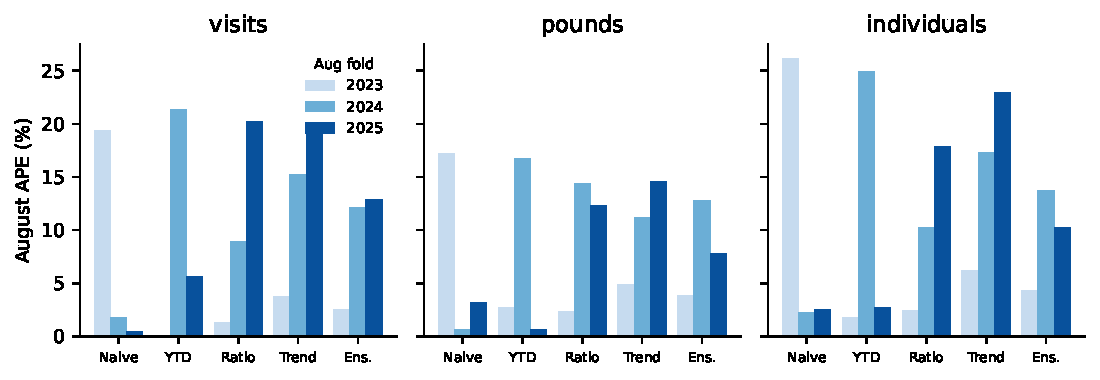
\includegraphics[width=0.95\textwidth]{required_models.pdf}
\caption{August absolute percentage error of the five reference models in each backtest fold
(Naive = seasonal naive, YTD = year-to-date growth, Ratio = July $\times$ Aug/Jul ratio,
Trend = trend + month regression, Ens.\ = robust median ensemble).}\label{fig:required}
\end{figure}

\noindent The pattern is consistent across outcomes. Growth-based models (YTD growth, ratio, trend)
win the 2023 ramp-up fold and then badly over-forecast the flat 2024--25 period, while seasonal naive
does the opposite. Damped YoY, which applies only half of recent growth, is the only reference model
that avoids large errors in every fold.

\section{Multi-agent model study}
Four specialist workflows ran in parallel. Each wrote models to the same interface, a function
from a cutoff-checked data slice to a statewide (or county) forecast, and was scored by the same
harness (Figure~\ref{fig:pipeline}).

\begin{figure}[H]\centering
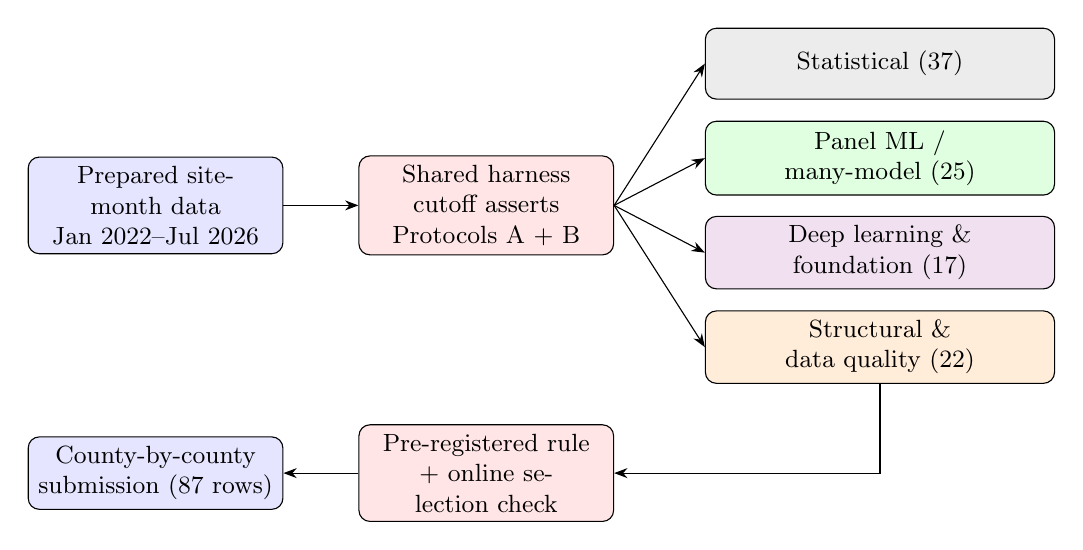
\begin{tikzpicture}[font=\small, >={Stealth},
  box/.style={draw, rounded corners, align=center, minimum height=9mm, text width=#1},
  box/.default=30mm]
\node[box, fill=blue!10]   (data) at (0,0)    {Prepared site-month data\\Jan 2022--Jul 2026};
\node[box, fill=red!10]    (h)    at (4.2,0)  {Shared harness\\cutoff asserts\\Protocols A + B};
\node[box=42mm, fill=gray!15]   (a1) at (9.2,1.8)  {Statistical (37)};
\node[box=42mm, fill=green!12]  (a2) at (9.2,0.6)  {Panel ML / many-model (25)};
\node[box=42mm, fill=violet!12] (a3) at (9.2,-0.6) {Deep learning \& foundation (17)};
\node[box=42mm, fill=orange!15] (a4) at (9.2,-1.8) {Structural \& data quality (22)};
\node[box, fill=red!10]    (sel)  at (4.2,-3.4) {Pre-registered rule\\+ online selection check};
\node[box, fill=blue!10]   (sub)  at (0,-3.4)   {County-by-county\\submission (87 rows)};
\draw[->] (data) -- (h);
\foreach \a in {a1,a2,a3,a4} {\draw[->] (h.east) -- (\a.west);}
\draw[->] (a4.south) |- (sel.east);
\draw[->] (sel) -- (sub);
\end{tikzpicture}
\caption{Study workflow. Numbers are the model variants each agent built (101 in total).}\label{fig:pipeline}
\end{figure}

\begin{description}
  \item[Statistical.] AutoETS, AutoARIMA, AutoTheta, AutoCES, and MSTL (Nixtla \texttt{statsforecast}) on
        raw and log scales; models of the year-over-year ratio series; a damped-YoY grid; and
        self-tuning damping chosen by inner rolling evaluation.
  \item[Panel ML / many-model.] Bottom-up forecasts at the county (87), food-bank (6), and site
        ($\sim$620) levels. These included simple local models, per-unit model selection in the style of
        the Databricks many-model framework, and global LightGBM and Ridge models trained on scale-free
        year-over-year log-ratios with past-only features.
  \item[Deep learning \& foundation.] Zero-shot Chronos-Bolt and Chronos-2 on statewide, food-bank,
        and county series, plus NHITS, NBEATS, and MLP networks trained on the county panel. The networks
        were retrained on a schedule that never uses data at or after the forecast origin.
  \item[Structural \& data quality.] Same-site growth, models of site entry and exit, reporting
        sites times per-site averages, cross-metric ratio models (pounds per visit, individuals per
        visit), and the diagnostics in Section~\ref{sec:diag}.
\end{description}

\begin{figure}[H]\centering
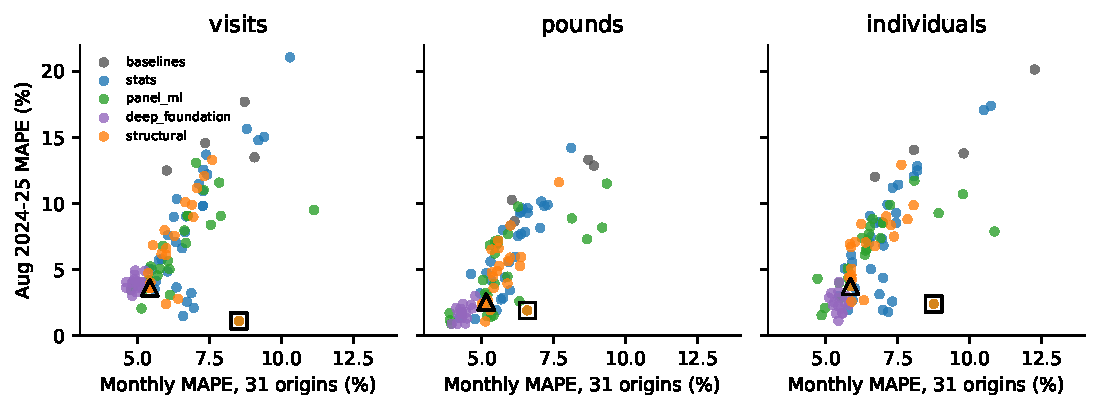
\includegraphics[width=0.97\textwidth]{leaderboard.pdf}
\caption{All 101 variants plus baselines. The x-axis is Protocol B MAPE and the y-axis is the
August 2024--25 MAPE; lower-left is better. The open square marks seasonal naive and the open
triangle damped YoY.}\label{fig:leader}
\end{figure}

\begin{table}[H]\centering\small
\caption{Best model from each agent by Protocol B MAPE (\%), compared with the baselines.}\label{tab:agents}
\begin{tabular}{lllrrr}
\toprule
Agent & Model & & Visits & Pounds & Individuals\\
\midrule
Baseline & Seasonal naive & & 8.52 & 6.59 & 8.75\\
Baseline & Damped YoY & & 5.43 & 5.16 & 5.86\\
Statistical & AutoTheta (log) & & 4.84 & 4.23 & 5.47\\
Panel ML & Per-county model selection & & 4.92 & \best{3.90} & \best{4.86}\\
Deep / foundation & MLP on county panel & & \best{4.60} & 3.96 & 5.11\\
Structural & Damped-YoY / cross-metric combo & & 5.44 & 5.02 & 5.81\\
\bottomrule
\end{tabular}
\end{table}

\paragraph{How much should we trust the winners?} The leaders improve on seasonal naive by two to four
points, but compared with damped YoY none of the differences is significant (paired tests over
31 origins, all $p>0.3$). The gains also come almost entirely from 2024, when the series levelled off.
To measure selection bias directly, we replayed the selection procedure out of sample: at each month
from January 2025 onward, we ranked all candidates using only their earlier errors, averaged the top
$k$, and scored the result (Figure~\ref{fig:honest}). Picking from 101 models was \emph{worse} than
using damped YoY or seasonal naive, so most of the apparent improvement is selection luck.

\begin{figure}[H]\centering
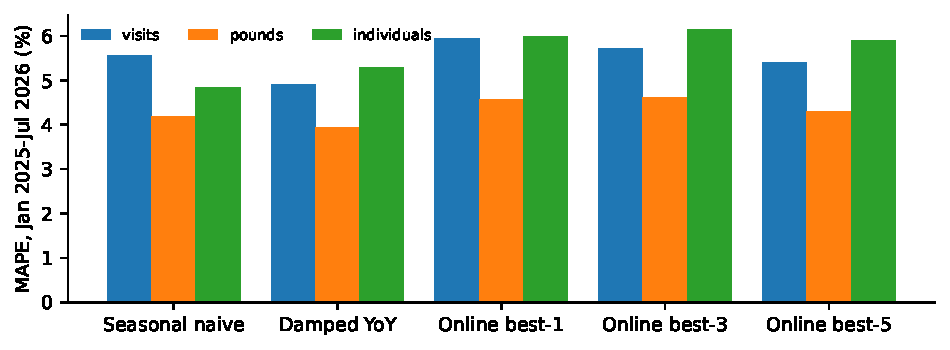
\includegraphics[width=0.8\textwidth]{honest_selection.pdf}
\caption{Out-of-sample replay of model selection, January 2025--July 2026 (19 origins).}\label{fig:honest}
\end{figure}

\section{Final model}
\subsection{From one recipe to county-by-county selection}
The study above pointed to simple, robust methods rather than a single sophisticated winner. Our first
candidate was an unweighted blend of three such forecasts, applied identically to every county:
seasonal naive (last year's August), damped YoY (last August scaled by half of recent three-month
growth), and per-county local-model selection (whichever of five simple local models had the lowest
error over the six months before the cutoff).

Because the submission is scored by county, we then examined where the county errors come from.
They are concentrated: four counties (Hennepin, Washington, Anoka, Dakota) account for half of all
absolute error and fifteen for 80\%. The counties forecast worst each had an identifiable site-level
event, which one recipe for every county handles poorly:
\begin{itemize}
  \item \textbf{Mille Lacs.} A new site opened in April 2026 with about 1{,}100 visits per month,
        roughly tripling the county; seasonal naive still anchors on August 2025 (512 visits).
  \item \textbf{Rice.} A one-off spike in August 2024 (8.1k vs.\ about 4k normally) became ``last August''
        for the 2025 forecast.
  \item \textbf{Scott and Dakota.} Individual sites with temporary jumps or erratic reporting.
\end{itemize}

We tested four county-tailoring variants under the same cutoff rules: forecasting each site and
summing to counties, the same with spike-capping, and per-county selection with a 12-month window. The
best was \textbf{county-by-county selection}, which became the final model. For each county it scores
five candidates (seasonal naive, damped YoY, local-model selection, the blend, and the recent
three-month mean) on that county's 12 one-month-ahead forecasts before the cutoff, and uses the
candidate with the lowest absolute error. All 12 scoring origins lie before the target month. When a
county has too little history to score all 12 (the August 2023 fold), the blend is used.

For August 2026 the visits forecasts used the recent mean in 33 counties, damped YoY in 21, the
blend in 14, seasonal naive in 10, and local-model selection in 8. Counties with a recent level
shift move to the recent mean; for example, Mille Lacs is forecast at 1{,}550 visits (July 2026:
1{,}623) instead of the blend's 991.

\subsection{County-level validation}
Table~\ref{tab:metrics} compares the final model with the blend on the full set of standard metrics
over the 31 monthly origins, and Table~\ref{tab:county} breaks county WAPE down by period.

\begin{table}[H]\centering\small
\caption{County-level metrics over 31 one-month-ahead origins (Jan 2024--Jul 2026): blend $\rightarrow$ final.}\label{tab:metrics}
\setlength{\tabcolsep}{4pt}
\begin{tabular}{lccc}
\toprule
Metric & Visits & Pounds & Individuals\\
\midrule
WAPE (\%) & 10.67 $\rightarrow$ \best{9.51} & 10.75 $\rightarrow$ \best{8.91} & 10.64 $\rightarrow$ \best{9.13}\\
County MAPE (\%) & 15.37 $\rightarrow$ \best{13.62} & 20.28 $\rightarrow$ \best{17.36} & 15.46 $\rightarrow$ \best{13.76}\\
Median APE (\%) & 9.71 $\rightarrow$ \best{8.42} & 10.93 $\rightarrow$ \best{9.80} & 10.11 $\rightarrow$ \best{9.10}\\
MAE & 306 $\rightarrow$ \best{272} & 15{,}958 $\rightarrow$ \best{13{,}214} & 941 $\rightarrow$ \best{807}\\
RMSE & 1{,}057 $\rightarrow$ \best{970} & 46{,}939 $\rightarrow$ \best{39{,}524} & 3{,}222 $\rightarrow$ \best{2{,}775}\\
Bias (\%) & $-3.0$ $\rightarrow$ \best{$-0.5$} & $-1.2$ $\rightarrow$ \best{$+0.1$} & $-2.7$ $\rightarrow$ \best{$+0.1$}\\
Statewide APE (\%) & 5.51 $\rightarrow$ \best{4.79} & 4.72 $\rightarrow$ \best{3.71} & 5.74 $\rightarrow$ \best{4.73}\\
\midrule
Months final better & 21 / 31 & 24 / 31 & 19 / 31\\
Wilcoxon $p$ (WAPE) & 0.036 & $<0.001$ & 0.006\\
\bottomrule
\end{tabular}
\end{table}

\begin{table}[H]\centering\small
\caption{County-level WAPE (\%) by period. Monthly columns are Protocol B; ``2026'' covers January--July 2026 only.}\label{tab:county}
\setlength{\tabcolsep}{4pt}
\begin{tabular}{llrrrrr}
\toprule
Outcome & Model & Aug 2023 & Aug 2024 & Aug 2025 & Monthly 2024--26 & Monthly 2026\\
\midrule
Visits & \textbf{Final (submitted)} & 20.7 & 8.0 & \best{6.1} & \best{9.5} & 12.3\\
 & Blend & 20.7 & \best{7.4} & 6.6 & 10.7 & 12.3\\
 & Seasonal naive & 36.6 & 10.5 & 9.4 & 15.3 & 13.6\\
\midrule
Pounds & \textbf{Final (submitted)} & 14.3 & \best{7.9} & \best{10.5} & \best{8.9} & 10.4\\
 & Blend & 14.3 & 10.2 & 11.5 & 10.8 & 10.4\\
 & Seasonal naive & 20.8 & 11.8 & 14.9 & 14.5 & 11.3\\
\midrule
Individuals & \textbf{Final (submitted)} & 20.3 & 8.1 & \best{4.1} & \best{9.1} & 11.7\\
 & Blend & 20.3 & \best{7.5} & 6.2 & 10.6 & 11.7\\
 & Seasonal naive & 34.3 & 10.1 & 9.3 & 15.4 & 13.0\\
\bottomrule
\end{tabular}
\end{table}

\begin{figure}[H]\centering
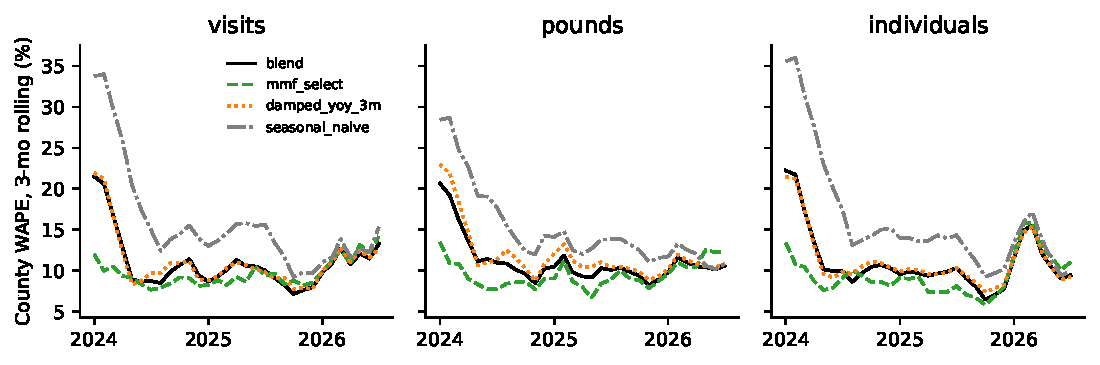
\includegraphics[width=0.97\textwidth]{county_backtest.pdf}
\caption{County-level WAPE over the monthly backtest (three-month rolling mean).}\label{fig:county}
\end{figure}

\noindent The final model improves every metric in Table~\ref{tab:metrics}, removes the blend's
systematic under-forecasting, and is significantly better in paired tests. It ties the blend in
2026 and is slightly worse in the August 2024 fold for visits and individuals ($+0.6$ points).
Because it was chosen from four variants after seeing their scores, its advantage is somewhat
optimistic; after a correction for the four comparisons, pounds and individuals remain significant
and visits becomes borderline ($p\approx0.14$). Relative to seasonal naive, the final model reduces
county error by about 40\% (the blend by about 30\%).

\subsection{Submitted forecast}
The 87-row file \texttt{Undergraduate\_}\allowbreak\texttt{Predictions\_Submit.csv} sums to the
statewide totals in Table~\ref{tab:final}. In the August 2023/2024/2025 backtests, the summed county
forecasts were within 10.8/1.4/3.8\% of the statewide actual for visits, 10.5/1.0/1.9\% for pounds,
and 15.6/1.2/1.6\% for individuals. Figure~\ref{fig:counties} compares the fifteen largest counties
with August 2025.

\begin{table}[H]\centering\small
\caption{Statewide sums of the submission with empirical 80\% ranges (quantiles of the final model's
signed statewide errors over the 31 monthly origins).}\label{tab:final}
\begin{tabular}{lrc}
\toprule
Outcome & August 2026 forecast & 80\% range\\
\midrule
Visits & 237{,}861 & 221{,}209 -- 258{,}297\\
Pounds & 12{,}994{,}439 & 12{,}186{,}624 -- 13{,}615{,}187\\
Individuals & 738{,}532 & 696{,}924 -- 802{,}298\\
\bottomrule
\end{tabular}
\end{table}

\begin{figure}[H]\centering
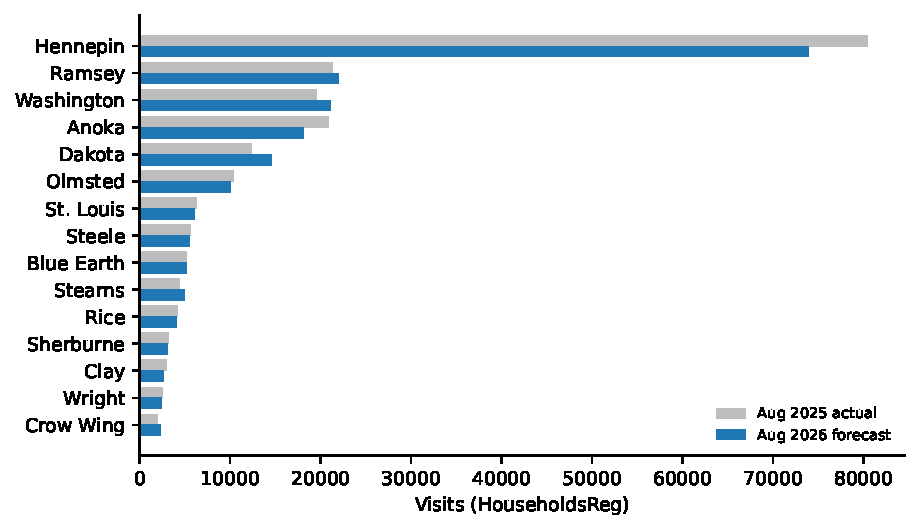
\includegraphics[width=0.75\textwidth]{top_counties.pdf}
\caption{Fifteen largest counties: August 2026 visit forecast vs.\ August 2025 actual.}\label{fig:counties}
\end{figure}

\section{Limitations}
\begin{itemize}
  \item There are only three historical August holdouts, and the first lies in a different regime.
        We add 31 monthly origins as a check, but those are not August-specific.
  \item With 101 variants tested, small differences are within noise; our recommendation relies on
        robustness rather than on the single best score.
  \item The blend and the county-by-county selection were each chosen after looking at results, from
        small sets of candidates. All candidates and their scores are reported for transparency.
  \item The data are a single snapshot. Later revisions to July 2026 reports cannot be observed,
        although every completeness diagnostic was normal.
  \item No external drivers (for example SNAP policy changes or prices) are included, because their
        availability before the cutoff could not be verified.
\end{itemize}

\section{Reproducibility}
All code is in \texttt{forecast\_august\_2026/}; run the commands below from that folder.
\begin{center}\small
\begin{tabularx}{\textwidth}{lX}
\toprule
Command & Output\\
\midrule
\texttt{python multiagent/harness.py} & reference models (Table~\ref{tab:required})\\
\texttt{python multiagent/<agent>/run.py} & each agent's predictions and \texttt{REPORT.md}\\
\texttt{python multiagent/combine.py} & pooled leaderboards and pre-registered selection\\
\texttt{python multiagent/honest\_selection.py} & out-of-sample selection replay\\
\texttt{python submission/make\_submission.py --team-id ID} & county backtest and the submission file\\
\texttt{python report/make\_figures.py} & all figures in this report\\
\bottomrule
\end{tabularx}
\end{center}
Every run writes a \texttt{cutoff\_check.txt} recording the assertions above.

\end{document}
